\section{Methodology}
%Redo research methodology section.
%Redo data analysis section.

\subsection{Research methodology}
%Research methodology description

% 1.2 Provide a problem statement with a strong hypothesis / Define your methodological approach 
Contemporary tools used to map network topologies such as Paristraceroute\cite{anomalies} and DiamondMiner\cite{diamond-miner} have improved on the original traceroute. However, these contemporary methods still have deficiencies, suggesting that there is still potential for these tools to be extended to mitigate these flaws. Thorough analysis of results from the literature and also from experimentation in a virtually implemented network will form the basis of the proposed improvements to the contemporary methods. 

In order to ensure the validity of the findings from experimentation in the virtual network lab and also create a testing framework which can be used to benchmark contemporary network scanning methods in the future, a multi-factorial approach will be employed. This includes a purposeful sample selection; topologies most commonly found in real world networks will be implemented, these include Bus, Ring, Mesh, Star, Tree and Hybrid configurations. This is to ensure that the selected sample population is representative of the overall population. Furthermore, a robust enumeration of macros across all possible network shapes will be explored, this will likely increase the available search space covered by the evaluation, through testing and evaluating the edge cases. Using this approach has the benefit of possibly highlighting potential flaws and unexpected behaviour of current methods, in a way that using conventional structures might not. By combining both  'real-world' and theoretical network topology structures, the implemented network lab has improved versatility and coverage of yielded data.  

% 3. State research design
\subsection{Research methods}
%Research methods description
Evaluation of the contemporary methods will be primarily quantitative. With the main measure of performance being focusing on the accuracy of the path tracking when tested on network structures in the virtual lab. Additionally, the execution time, packet loss handling  will also be taken into account.

They will be evaluated using ContainerLab \cite{containerlab} which is an open source network emulator which allows the creation of virtual network environments, leveraging the powerful docker framework, it supports containerized router images of products offers by major companies such as Cicso, Juniper and Dell. For the purpose of this research project, Alpine Linux will be used for the container images, due to it's low running constraints compared with similar Linux distributions such as Debian\cite{alpine} and open-source code base. This mitigates any potential memory concerns when simulating more complex network topologies. Furthermore, by evaluating the contemporary tools in a virtual network lab the experiment variables are fully controllable, allowing for repeatable results and avoidance of external interference. By using a virtual environment the possibility of numerous results being collected for each configuration are ensured, allowing statistical analysis of the results to be carried out. This further increases the validity of the evaluation. Additionally, by simulating the network topologies ethical implications of evaluating performance on the real-world internet are avoided. 

% 4. Discuss specifics of data collection and methodology

% 5. Justify methods used - mention limitations, strengths and weaknesses.

\subsection{Virtual Network lab}
To facilitate evaluation of the contemporary network scanning tools, a virtual network lab has been created. The implemented virtual network lab was created inside a virtual machine running the Debian based Linux Operating System  Kali Linux. 

Using this approach allows for an isolated testing environment, avoiding external factors which could interfere with the experimental results. Furthermore, by employing a virtual lab complete control and configuration of the experimental variables is ensured. Due to this the experimental results can be replicated a number of times, increasing the validity of the findings. 

Additionally, due to the portability of virtual machines across varying Operating systems, the configuration and findings from this research can be readily built upon and revised, encouraging more work in this area.

In order to measure and compare the performance of tools utilised to map network topologies in an objective manner, a standardised testing environment should be employed. Creation and design of this given testing environment will be based upon a multi-factorial approach; by utilising structures which are representative of real world network topology, using configurations such as so-called "star" and "bus" topologies will ensure a realistic measurement of expected performance with a high probability of confidence due to their prevalence across many varying topologies. 

Additionally, in conjunction with the practical real-world approach, a robust enumeration of all possible network shapes will be employed to increase the available performance search space of each tool in topology measurement. Utilising this stochastic approach allows for potential edge cases to be identified, possibly highlighting previously unknown design flaws/weaknesses in a given tool. 

\subsection{Topology models}
Below, the network topology models used in the creation of the virtual network lab will be described and outlined, in order to justify the rationale and decision making process in creation of the final models. 

\subsubsection{Ring topology}
A Ring topology comprises of a set of nodes connected in a circular manner. In other words, each node is connected to precisely two other nodes. This results in a singular uninterrupted route for data to travel through each node. Internet service providers employ ring network's for the "backbone" of many of their networks \cite{ring_network}, furthermore it is also commonly found on local area networks and Intranets. Due to it's circular nature it has a "low transmission efficiency and high delay", for a packet to traverse the entire network it must first past through every preceding node. This also highlights its other deficiency; it's unreliability. If a node or link breaks in the network, the nodes beyond are unreachable. \cite{ring_network}

\subsubsection{Bus topology}
A bus topology comprises of nodes which are directly connected to a shared link, called a "bus". As a consequence of this, nodes in the network are not directly connected to one another with the bus carrying all of the transmitted data between each node in the network. Due to the simplicity of it's design the bus topology is relatively straightforward to establish and also has a low setup cost; however it faces problems with scalability, due for the potential for collisions to occur between transmitted packets along the shared bus negatively impacting network performance. Furthermore, the bus topology lacks reliability, if the bus link is damaged/broken the entire network could go down. 

\subsubsection{Star topology}
A star topology comprises of a central node, with terminal nodes radially connected outwards. In order for data to be transferred  between the terminal nodes in the network, it must pass through the central node, thus much like the bus topology, direct data transfer between the terminal nodes is not possible. \cite{star_zig} Due to the independent connection of each node to the central node, the topology is relatively fault tolerant as one link braking will not impact the other connections in the network. Furthermore, should a potential fault occur, it can be more readily dealt with, due to the increased ability to identify and distinguish sources of problems in the network. Star topologies are commonly found across many different use-cases and contexts; such as a  home network, where each device is directly and independently connected to a centralised router/hub. 

\subsubsection{Mesh topology}
Mesh topologies are composed of nodes which are connected directly and non-hierarchically to one another. They can be classified as either partially connected or fully connected, whereby nodes are partly connected and fully connected respectively to form a "mesh" structure. Due to the mutual connections between every node in the network, there is a lack of dependancy on any particular node or connection. The mutual connectivity between each/many of the nodes in a mesh topology makes it fault-tolerant and also allows on-the-fly distribution of load on the network. \cite{mesh_paper}

\subsubsection{Tree topology}
A tree topology is a form of hybrid network topology, it consists of both star and bus networks. It is composed of star networks connected together through a shared bus network. \cite{tree_book} Furthermore, due to the characteristics of it's component topologies, star and bus, the tree topology is well suited to be used for networks that span "large geographical areas" \cite{Qos_simulation}. 

By combining star and bus topological structures, the tree topology can benefit from the strengths of both component topologies; the efficiency and robustness of star networks and also the simplicity and low overhead cost of bus networks.

Tree network topologies can be characterised as both "Regular" and "Random". A regular tree network's topology structure is specified by the branching, $d$, and also the number of generations, $G$ \cite{tree_nature}. With the total number of nodes and peripheral nodes ($N$ and $N_p$ respectively) given by the following:

\begin{equation}
    N = \frac{d^{G+1}-1}{d-1}
\end{equation}

\begin{equation}
    N_d = d^G
\end{equation}

\subsubsection{Hybrid topology}
Hybrid topologies are composed of multiple varying simple topologies which combine to create new composite structures. as previously mentioned the tree topology is one such example of a hybrid topology; whereby star and bus topologies combine to create a new more complex structure. Theoretically, there are infinite combinations of simple topologies which combine to create hybrid topologies, due to there being no defined size and complexity constraints. However, in real-world network's there are a set of commonly found hybrid topology configurations which form the vast majority of all networks.

Real world examples of hybrid network topologies include a University campus intranet or in an enterprise context. 

\subsection{Real-world topologies}
\subsubsection{Topology zoo}
"[The] Internet Topology Zoo is a store of network
data created from the information that network operators make
public." \cite{topology_zoo} The Internet Topology Zoo is a project carried out at the University of Adelaide by Knight et al, aiming to create an accurate database of real-world network topologies from publicly available information. It has the distinction of not being measured by network scanning tools such as traceroute \cite{jacobson1989traceroute}, therefore it avoids the potential innacuracies which using these tools can entail. Furthermore, due to the information being gathered using this approach, many of the topologies stored in the database have additional metadata. This provides not only a more rich and descriptive abstraction of network structures but can also enable discovery of further topologies. 

\begin{figure}
\centering
\begin{subfigure}{.5\textwidth}
    \centering
    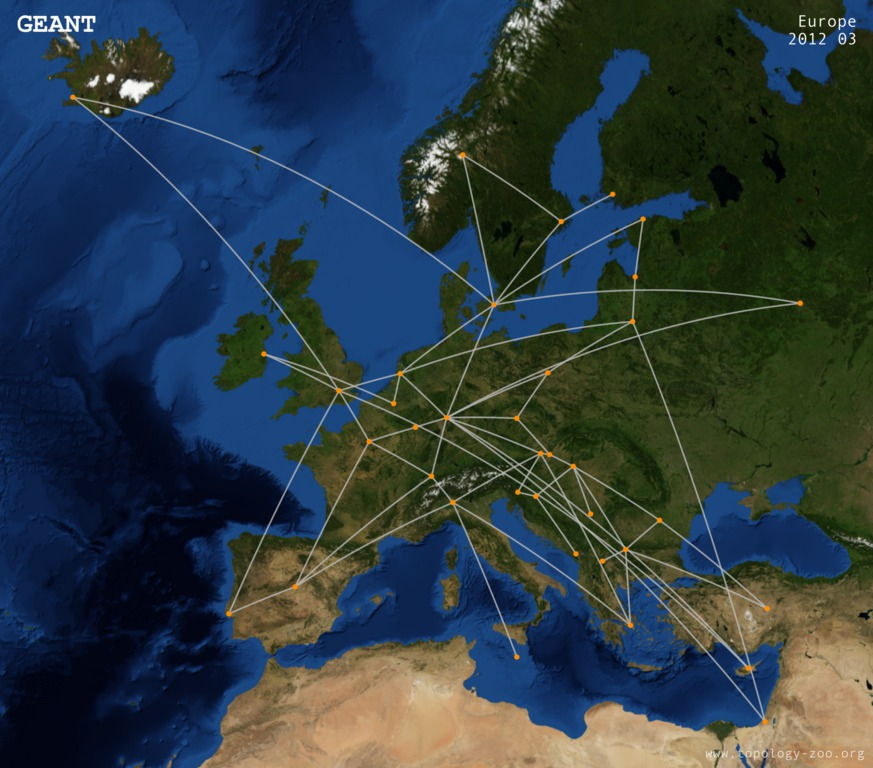
\includegraphics[width=0.7\linewidth]{images/real-world/GEANT_2012.jpg}
    \caption{GEANT (2012) \cite{topology_zoo}}
    \label{fig:GEANT}
\end{subfigure}%
\begin{subfigure}{.5\textwidth}
    \centering
    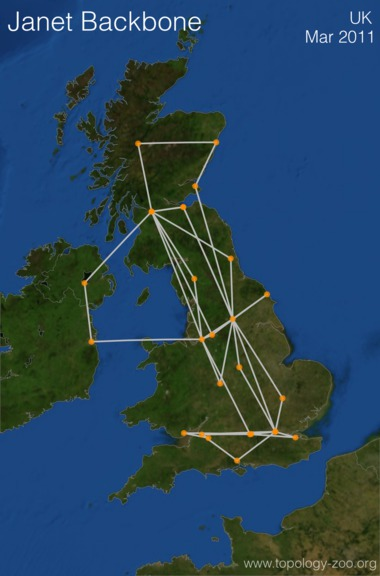
\includegraphics[width=0.5\linewidth]{images/real-world/Janetbackbone_2011.jpg}
    \caption{Janet Backbone (2011) \cite{topology_zoo}}
    \label{fig:janet_backbone}
\end{subfigure}
\caption{Example Backbone primary networks from the Internet Topology Zoo database}
\label{fig:test}
\end{figure}

Topologies are not only visualised but also captured in the GML graph exchange format, enabling straightforward processing of the topologies in a scripting language such as python. 

\begin{figure}
\centering
\begin{subfigure}{.5\textwidth}
    \centering
    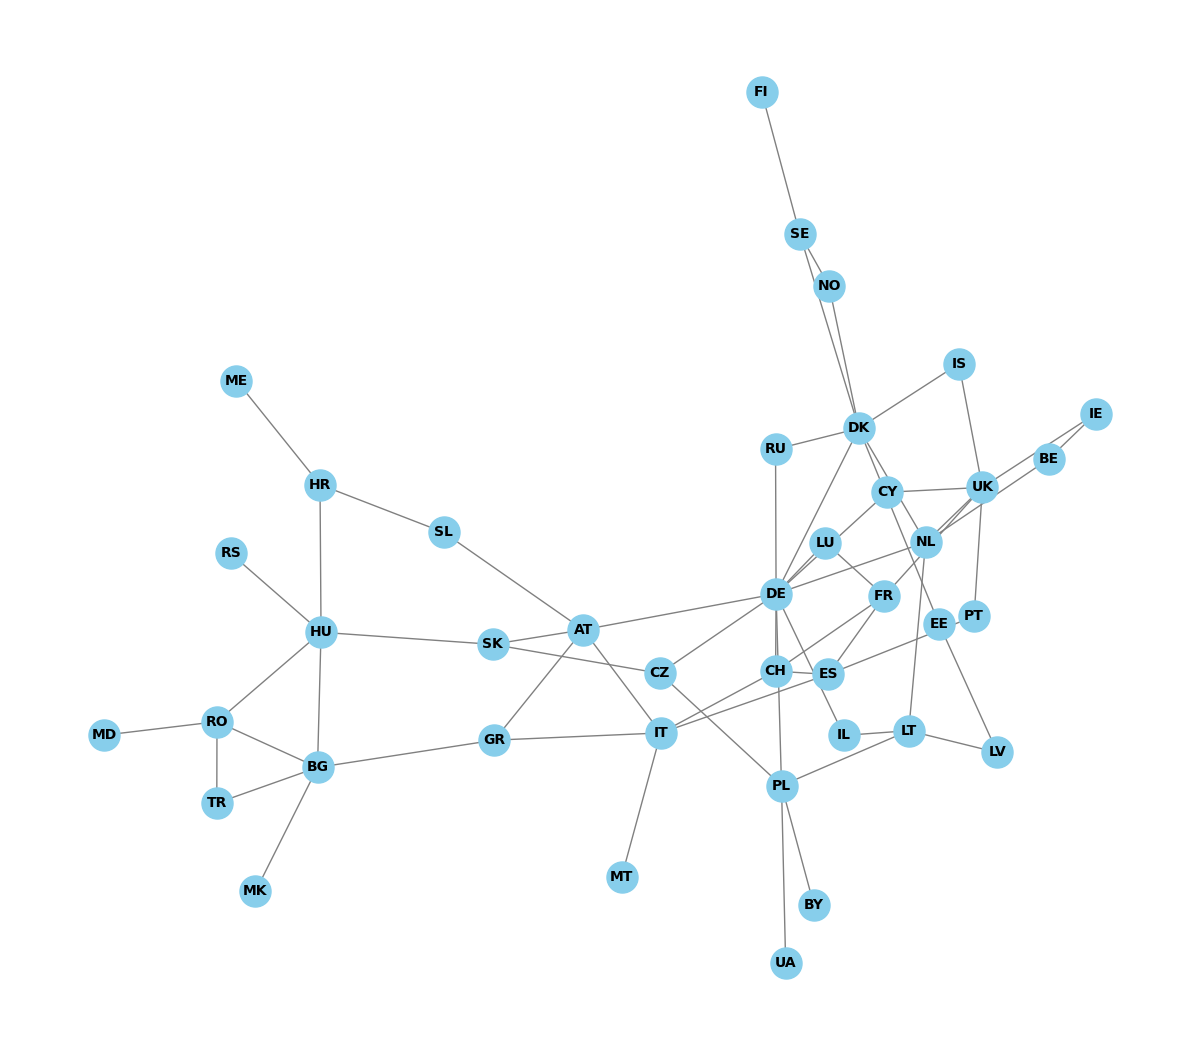
\includegraphics[width=0.7\linewidth]{images/real-world/geant_plot.png}
    \caption{GEANT (2012) \cite{topology_zoo}}
    \label{fig:GEANT_plot}
\end{subfigure}%
\begin{subfigure}{.5\textwidth}
    \centering
    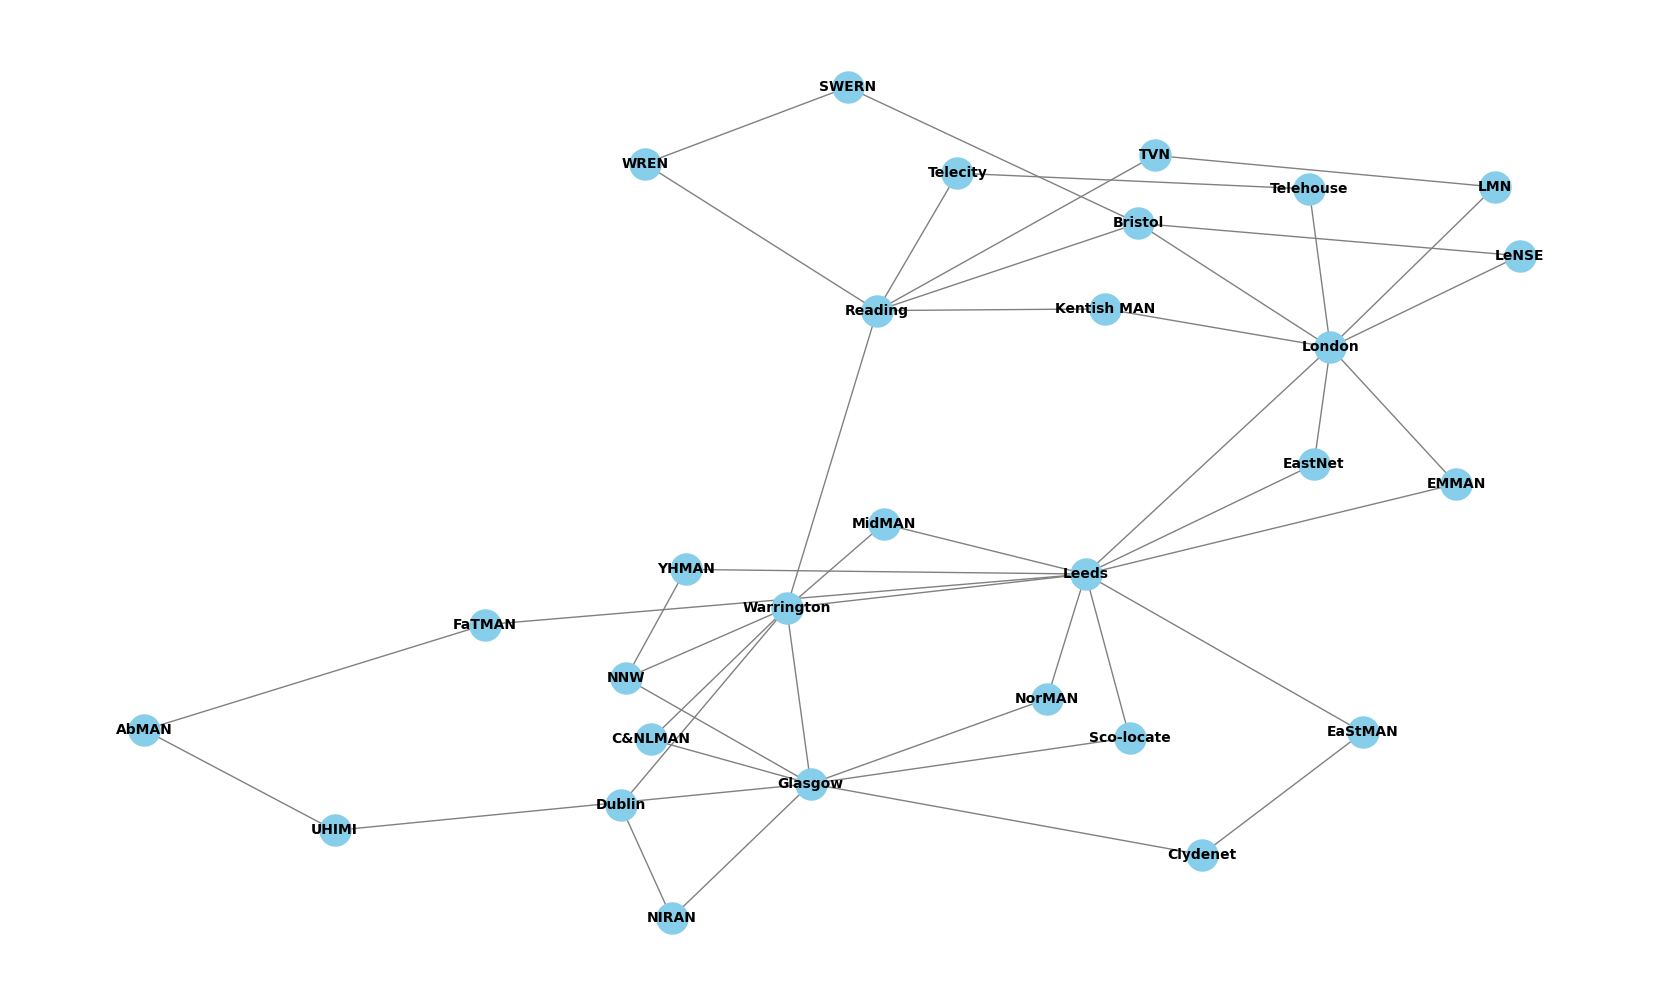
\includegraphics[width=0.7\linewidth]{images/real-world/janet_plot.png}
    \caption{Janet Backbone (2011) \cite{topology_zoo}}
    \label{fig:janet_backbone_plot}
\end{subfigure}
\caption{GEANT and Janet Backbone topologies imported and plotted directly using python}
\label{fig:test}
\end{figure}

By analysing and evaluating contemporary network scanning tools on simulated models of real-world networks, meaningful conclusions can be drawn from experimental results. The practical application of these tools will be tested, in the  environment they were intended to be used for. Furthermore, with a wide variety of different real-world topologies are available through the Internet Topology zoo, extensive and exhaustive testing can be carried out. 

\subsection{Stochastic topologies}
With the aim to implement randomly generated network topologies for the purpose of evaluation in the virtual network lab, several frameworks are proposed.

\subsubsection{Basic approach}
Following an elementary approach which is concerned with the basic 'building-blocks' of a network topology, one can identify these as the number of nodes, the number of links each node has, the origin node and target node of each link. 

\subsubsection{Individual topologies}
Another approach could be to vary the structure of a specific individual topology type at random, based on their defined character and attributes. This would likely be of more interest using more complex structures such as a 'tree' topology, which is expressed through the parameters $d$, $G$.

\subsubsection{Topology library}
A further approach which could be employed would be to have a set of varying basic topologies to form a topology library. This set would include bus, star, mesh and ring topologies of differing sizes and structures. The parameters for random generation of the topology structure in this instance would be the topologies which are to be selected at random from the set, a random number of times, and also how each of these selected topologies would be connected to each other to form a complete logical structure. This approach would have the benefit of being more representative of structures actually found in real-world networks, as opposed to purely random configurations. This is due to being synthesised from component topologies which are actually utilised in the real-world for their individual characteristics.

\begin{figure}
    \centering
    \begin{lstlisting}
import random 

# Individual topology variants
ring = [ring_1, ring_2, ring_3]
bus = [bus_1, bus_2, bus_3]
star = [star_1, star_2, star_3]
mesh = [mesh_1, mesh_2, mesh_3]

# Main topology set
topology_set = [ring, bus, star, mesh]

# Generated topology
generated_topo = []

# Parameter definition
n = 3 # Number of topologies to be selected

for i in range(n):
    # topologies which are to be selected at random from the topology_set, [j,k]
    j = random.randint(len(topology_set)-1)
    k = random.randint(len(topology_set[j])-1)

    # Append to generated topology 
    generated_topo.append(topology_set[j][k])

\end{lstlisting}
    \caption{Example python implementation of random selection from topology library to create new topologies}
    \label{fig:topology_library}
\end{figure}

\subsubsection{Erdos-Renyi Model}
The Erdos-Renyi model \cite{Erdos_renyi_origin} covers two similar mathematical models proposed by Erdos, Renyi and seperately Gilbert \cite{gilbert_background}. They can both be used to randomly generate graphs with a fixed number of nodes $n$. However, the models differ in their approach to creating links between given nodes in the generated graph. The first variant is defined through $G(n,M)$, whereby a graph is generated by randomly selecting one individual instance from the collection of all possible graphs defined by having $n$ nodes and $M$ edges. The random graph selection is uniform, thus each outcome is equally likely to occur. 

\begin{equation}
    G(n,M)
\end{equation}

\begin{algorithm}
\caption{\( G(n, M) \) Erdős-Rényi Model}\label{alg:GnM}
\begin{algorithmic}[1]
\State \textbf{Input:} Number of nodes \( n \), number of edges \( M \)
\State \textbf{Output:} Random graph \( G(V, E) \)

\State \textbf{Step 1:} \textbf{Initialization}
\State Create a set of \( n \) nodes \( V = \{v_1, v_2, \dots, v_n\} \).
\State Initialize an empty set of edges \( E = \emptyset \).

\State \textbf{Step 2:} \textbf{Edge Selection}
\State Let \( \mathcal{P} \) be the set of all possible pairs of nodes \( \{(v_i, v_j) \mid 1 \leq i < j \leq n\} \).
\State Randomly select \( M \) unique pairs from \( \mathcal{P} \) without replacement.

\State \textbf{Step 3:} \textbf{Edge Addition}
\For{each selected pair \( (v_i, v_j) \)}
    \State Add the edge \( (v_i, v_j) \) to the edge set \( E \).
\EndFor

\State \textbf{Step 4:} \textbf{Output the graph}
\State The graph \( G(V, E) \) consists of the node set \( V \) and the edge set \( E \).
\end{algorithmic}
\end{algorithm}

The second variant, proposed by Gilbert is defined through $G(n,p)$, whereby a graph is randomly created by linking labeled nodes in a random manner, according to the parameter $p$ an edge will be added in the graph between two nodes. 

\begin{equation}
    G(n,p)
\end{equation}

\begin{equation}
    p^M(1-p)^{(n \atop 2)-M}
\end{equation}

\begin{algorithm}
\caption{\( G(n, p) \) Erdős-Rényi Model}\label{alg:Gnp}
\begin{algorithmic}[1]
\State \textbf{Input:} Number of nodes \( n \), probability \( p \)
\State \textbf{Output:} Random graph \( G(V, E) \)

\State \textbf{Step 1:} \textbf{Initialization}
\State Create a set of \( n \) nodes \( V = \{v_1, v_2, \dots, v_n\} \).
\State Initialize an empty set of edges \( E = \emptyset \).

\State \textbf{Step 2:} \textbf{Edge Creation}
\For{each pair of nodes \( (v_i, v_j) \) with \( 1 \leq i < j \leq n \)}
    \State Generate a random number \( r \) uniformly distributed between 0 and 1.
    \If{\( r \leq p \)}
        \State Add the edge \( (v_i, v_j) \) to the edge set \( E \).
    \EndIf
\EndFor

\State \textbf{Step 3:} \textbf{Output the graph}
\State The graph \( G(V, E) \) consists of the node set \( V \) and the edge set \( E \).
\end{algorithmic}
\end{algorithm}


A the model is probabilistic, the parameter $p$ exists on the range 0 to 1; intuitively as $p$ increases the likelihood of generating graphs with more links increases, with the converse also being true.

\begin{figure}
    \centering
    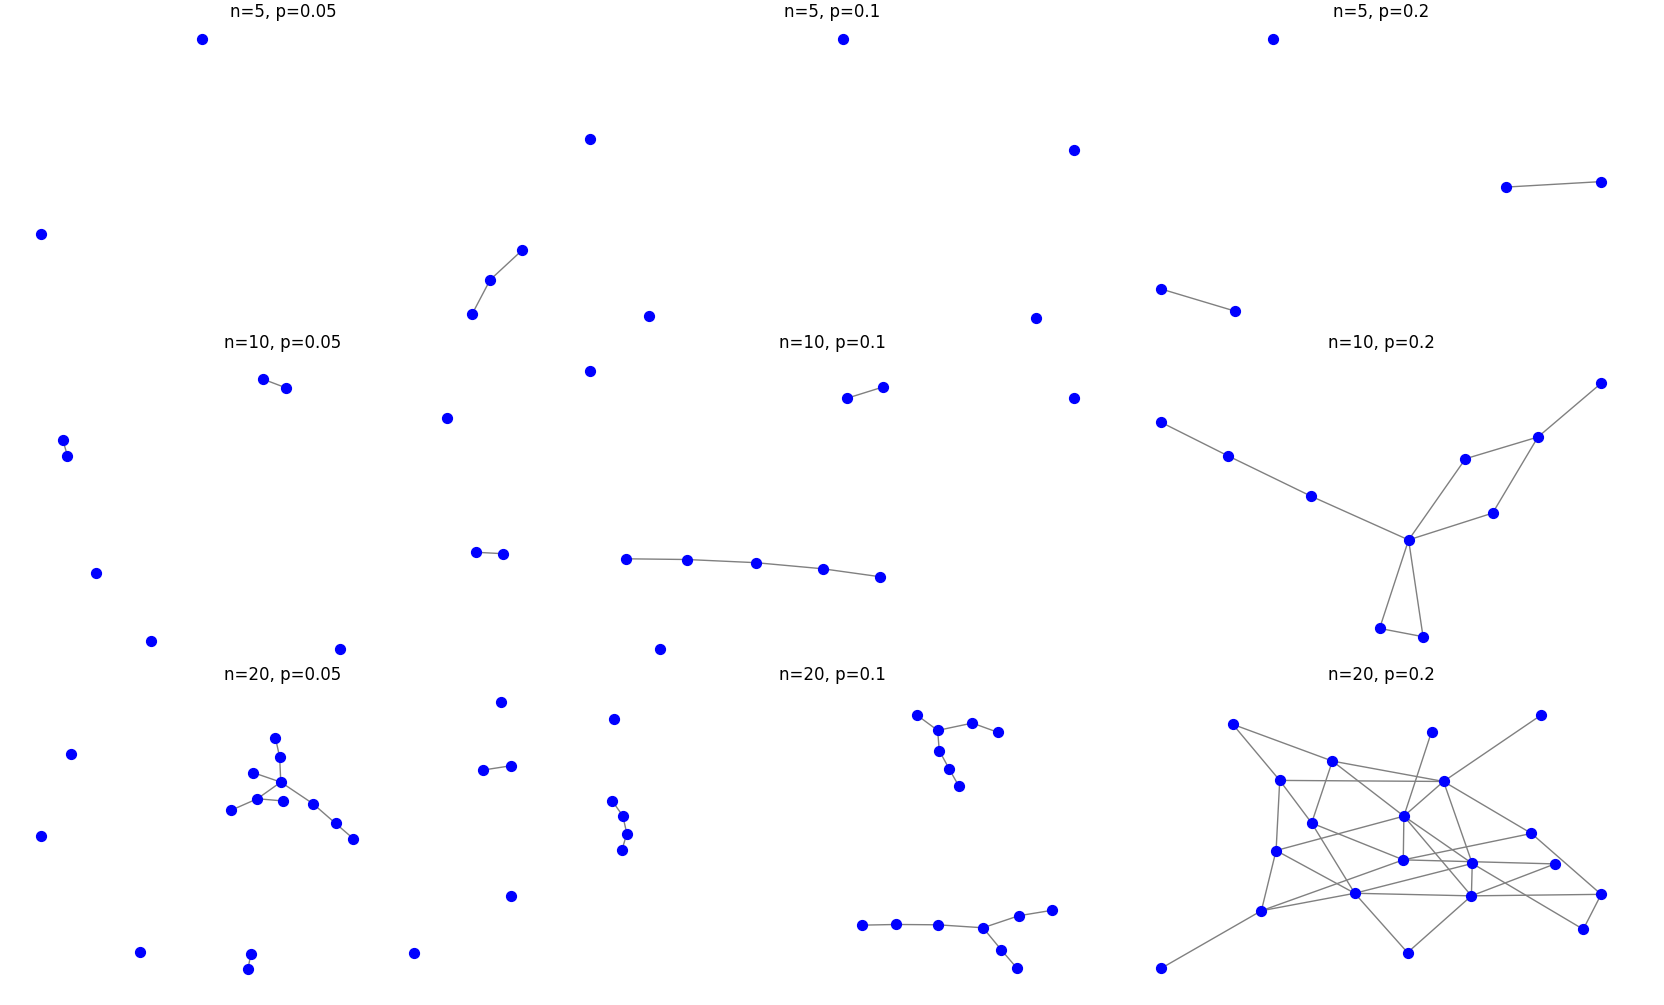
\includegraphics[width=0.75\linewidth]{images/ER/low_prob/low_prob_5,10,20.png}
    \caption{Graph topology plots with varying numbers of nodes, $n$ and probabilities $p$ to illustrate the effect of these parameters on network structure.}
    \label{fig:low_prob_5,10,20}
\end{figure}

\begin{figure}
    \centering
    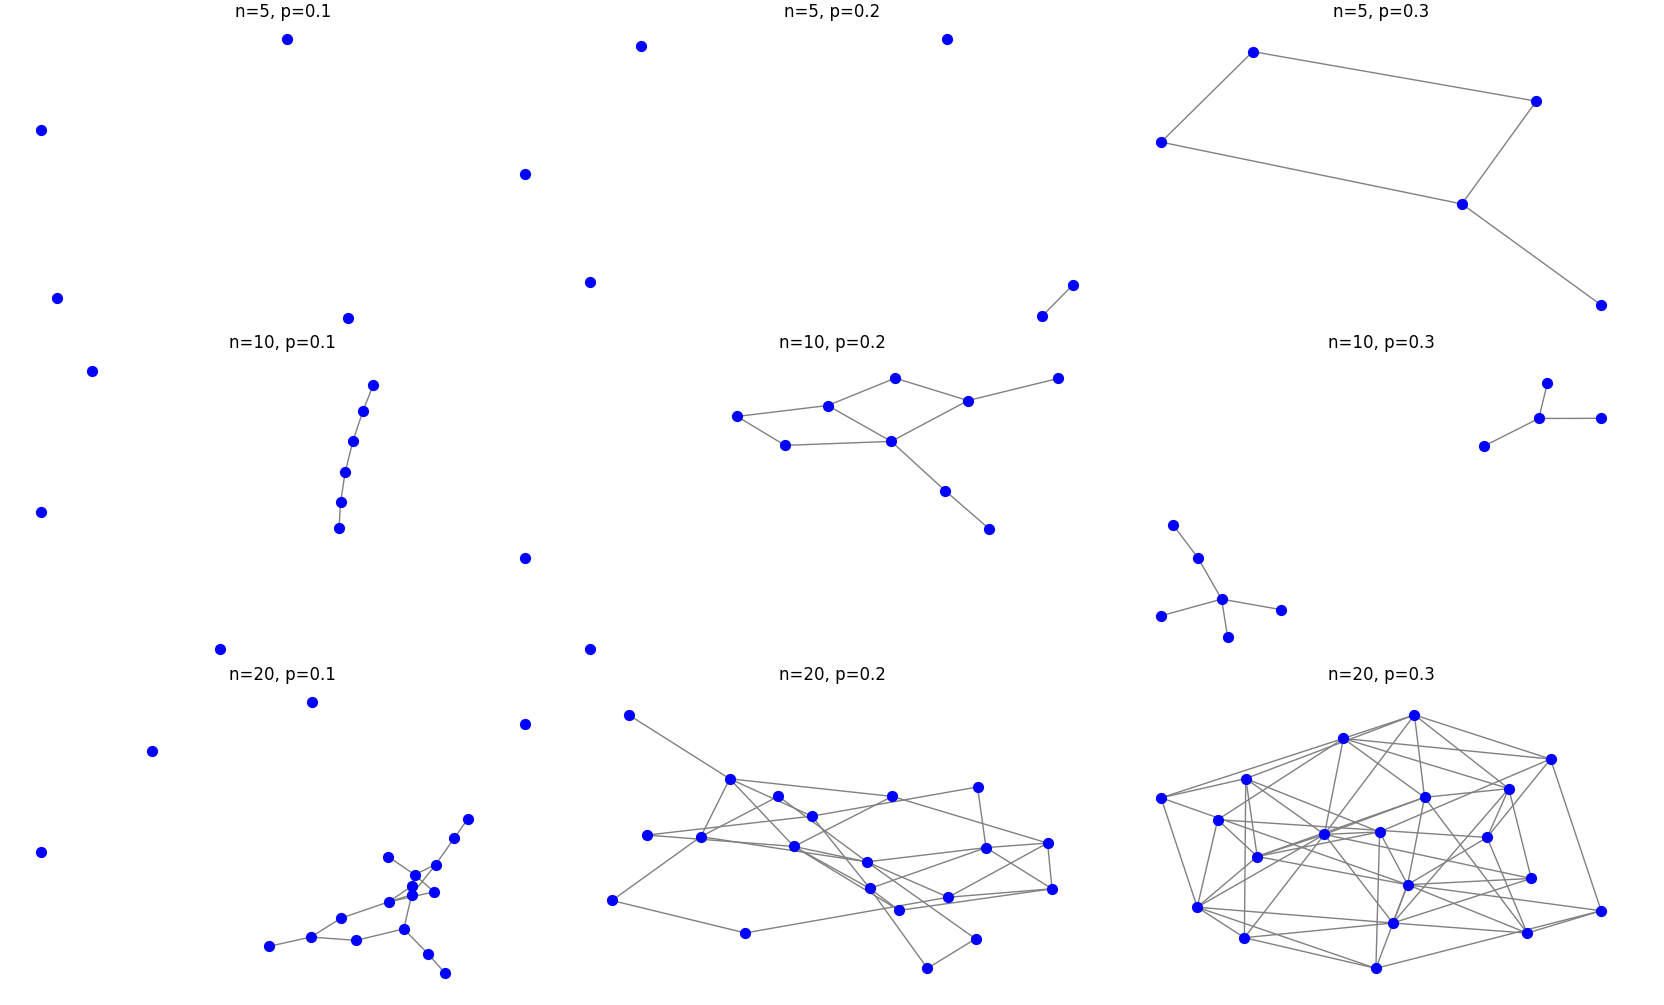
\includegraphics[width=0.75\linewidth]{images/ER/5,10,20.png}
    \caption{Graph topology plots with varying numbers of nodes, $n$ and probabilities $p$ to illustrate the effect of these parameters on network structure.}
    \label{fig:5,10,20}
\end{figure}

\begin{figure}
    \centering
    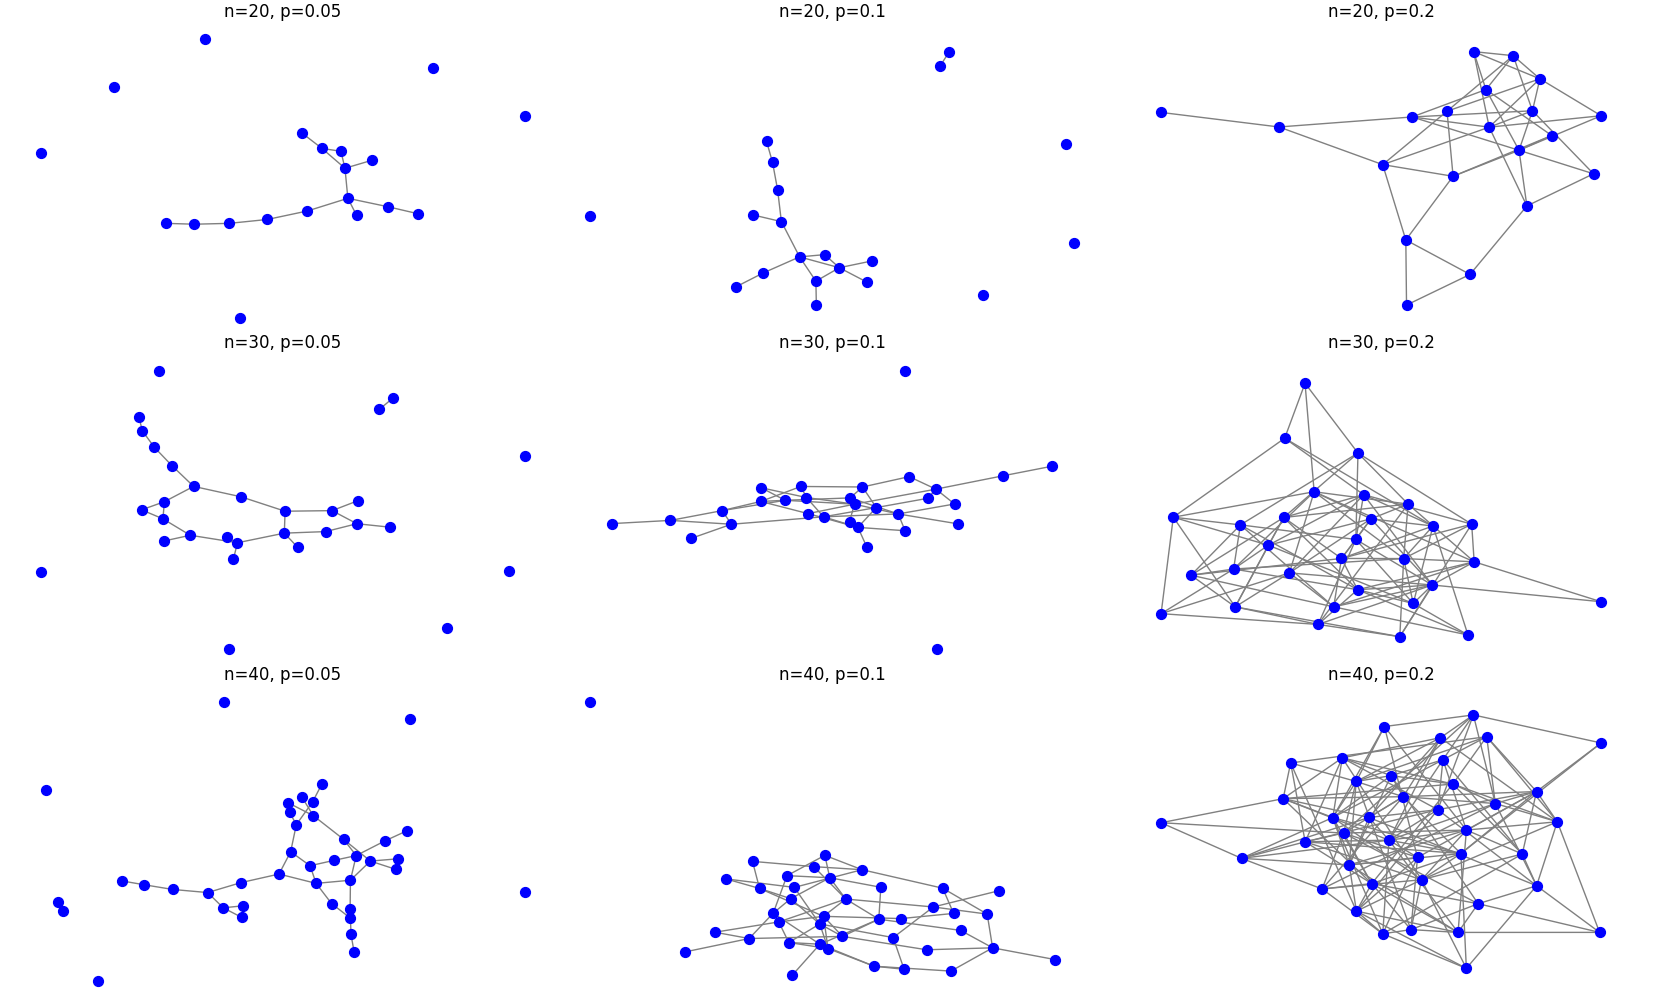
\includegraphics[width=0.75\linewidth]{images/ER/low_prob/low_prob_20,30,40.png}
    \caption{Graph topology plots with varying numbers of nodes, $n$ and probabilities $p$ to illustrate the effect of these parameters on network structure.}
    \label{fig:low_prob_20,30,40}
\end{figure}

\begin{figure}
    \centering
    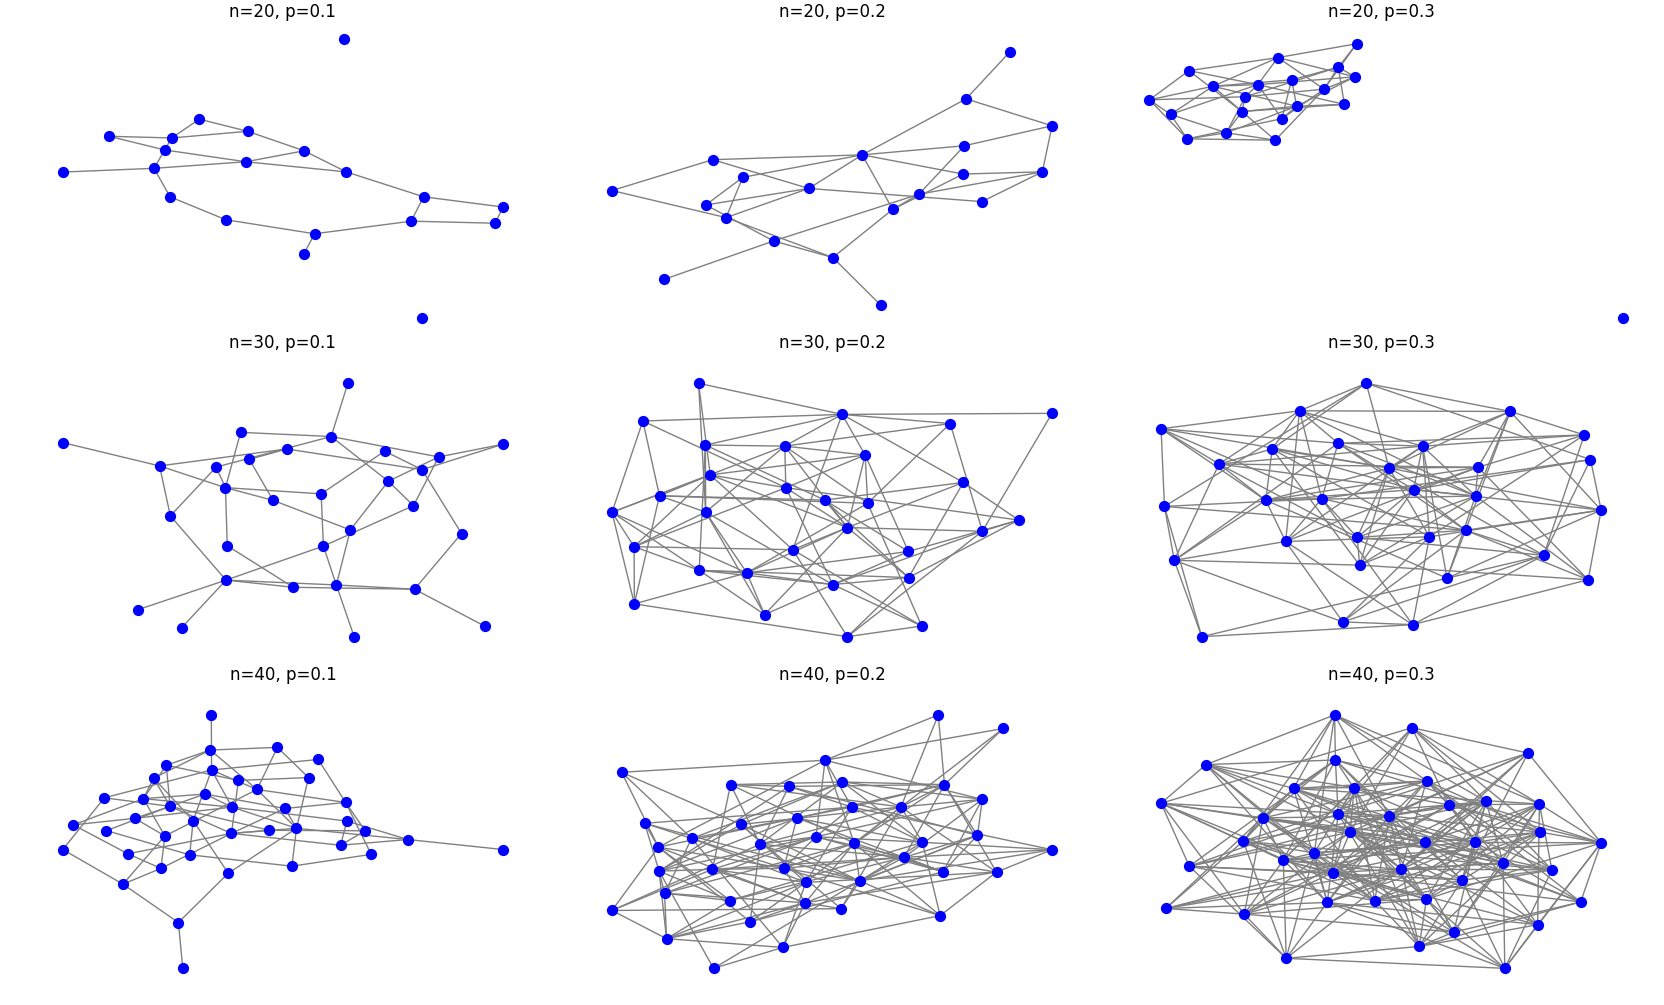
\includegraphics[width=0.75\linewidth]{images/ER/20,30,40.png}
    \caption{Graph topology plots with varying numbers of nodes, $n$ and probabilities $p$ to illustrate the effect of these parameters on network structure.}
    \label{fig:20,30,40}
\end{figure}

For the purposes of network topology generation, the G(n,M) is the most straightforward implement. Due to the every node in the network having at least one link to another node, avoiding unconnected nodes and separated networks. However, one way to circumvent these potential issues would be to prune the outlying nodes and keep the largest network. 

\subsubsection{Barabasi-Albert Model}

%Discuss how it is likened to real-world networks such as the WWW and social networks, think it would be highly applicable for this use-case.
The Barabasi-Albert models is an algorithm which  produces random scale-free networks, the networks are generated utilising a preferential attachment approach. Whereby the more links a given node has to other nodes, the higher the probability it will get more new links. A node's degree is the probability of garnering new link's with other nodes.

Initially the network starts with a network of $m_0$ nodes, at each step a new node is added with $m$ edges which link it to $m$ different nodes. The probability that a new node will connect to an existing node $i$ is given by \ref{eq:3}, where $k_i$ is the degree of node $i$, and the sum is over all existing nodes $j$. \cite{Albert_barabasi_2002} 


\begin{equation} \label{eq:3}
    p_i = \frac{k_i}{\Sigma_jk_j}
\end{equation}

\begin{figure}
    \centering
    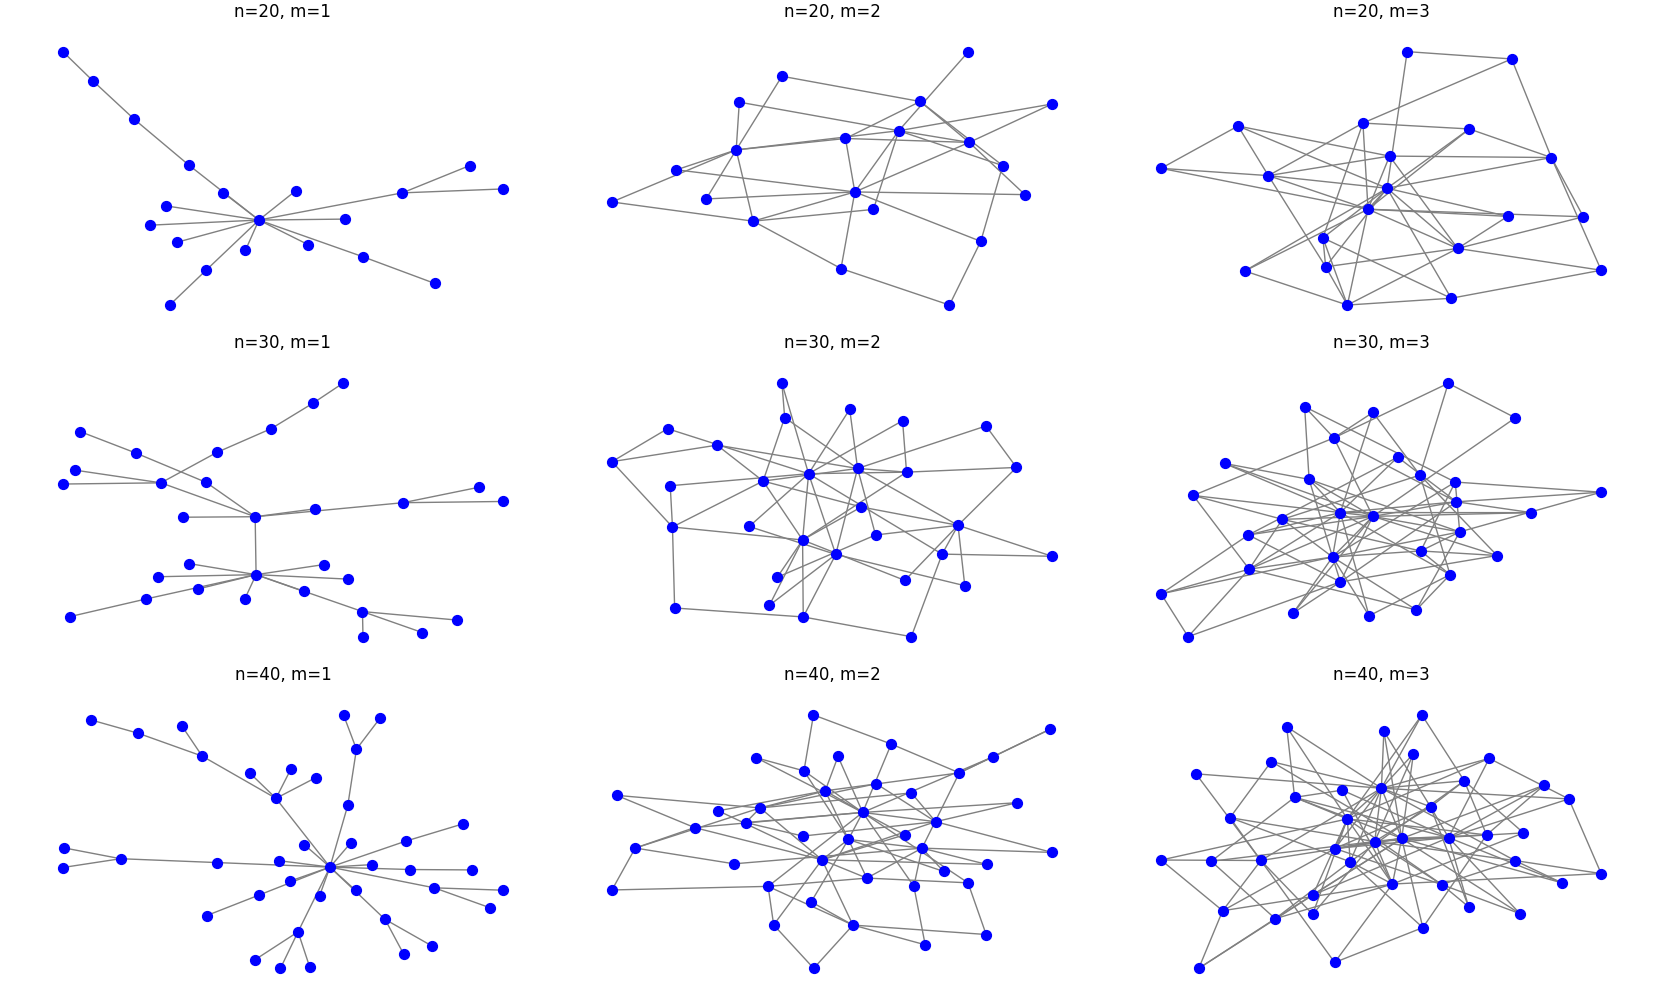
\includegraphics[width=0.75\linewidth]{images/BA_9.png}
    \caption{9 different randomly generated networks using the BA model algorithm, each with varying n and m values to illustrate the impact of each parameter}
    \label{fig:BA_9}
\end{figure}

\begin{algorithm}
\caption{Barabási-Albert (BA) Model Algorithm}\label{alg:BA}
\begin{algorithmic}[1]
\State \textbf{Input:} Initial number of nodes $m_0$, number of edges to attach $m \leq m_0$, total number of nodes $N$
\State \textbf{Output:} Scale-free network with $N$ nodes
\State

\State \textbf{Step 1:} \textbf{Initialization}
\State Create an initial network with $m_0$ nodes and connect every node to every other node (complete graph).

\State \textbf{Step 2:} \textbf{Growth}
\For{$i = m_0 + 1$ to $N$}
    \State Add a new node $i$ with $m$ edges.
    \State Connect the new node $i$ to $m$ existing nodes chosen with probability proportional to their degree.
    \For{each existing node $j$}
        \State Calculate the probability $\Pi(j)$ that node $i$ connects to node $j$:
        \[
        \Pi(j) = \frac{k_j}{\sum_{l} k_l}
        \]
        where $k_j$ is the degree of node $j$ and the sum is over all existing nodes $l$.
    \EndFor
\EndFor

\State \textbf{Step 3:} \textbf{Repeat}
\State Repeat the growth process until the network contains $N$ nodes.

\State \textbf{Step 4:} \textbf{Output the network}
\State Return the generated scale-free network.
\end{algorithmic}
\end{algorithm}

\subsubsection{Python Implementation}
Each of these approaches could be facilitated by implementing them in python to create custom topology definition files in such a way which can then be parsed by containerlab to deploy and host the topologies virtually. 
The python library networkx \cite{networkX} has stochastic graph generating functions which can implement the Erdos-Renyl and Barabasi-Albert models, reducing overall development time and ensuring accurate and efficient code. 

\subsection{Generated and Real-world Topologies comparison}
To verify the validity of the generated topologies they will be compared with real-world topologies found from the Internet Topology Zoo database. Furthermore, this will be used as the basis of selection from the different topology generation methods mentioned previously. The correlation between them will be measured in several different ways to ensure a rigorous and comprehensive approach.

\subsubsection{Graph Isomorphism}
Given two graphs 

\begin{equation}
    (u,v) \in E_1 \Leftrightarrow (f(u),f(v)) \in E_2
\end{equation}

\subsubsection{Degree Correlation}

\begin{equation}
    r = \frac{\sum(x_i - \hat{x})(y_i-\hat{y}}{\sqrt{\sum}(x_i-\hat{x})^2\sum(y_i-\hat{y})^2}
\end{equation}


%\subsubsection{Spectral Comparison}
%\subsubsection{Clustering Coefficient Comparison}

\subsubsection{Distribution of shortest path lengths}


\begin{figure}
\centering
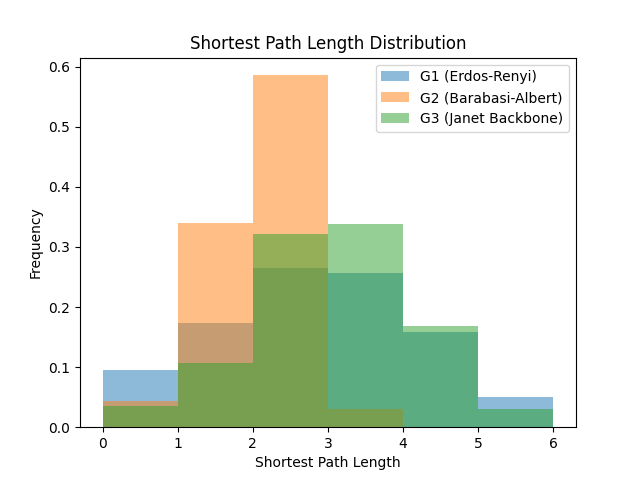
\includegraphics[width=.3\textwidth]{images/topo_comparison/janet1.png}\hfill
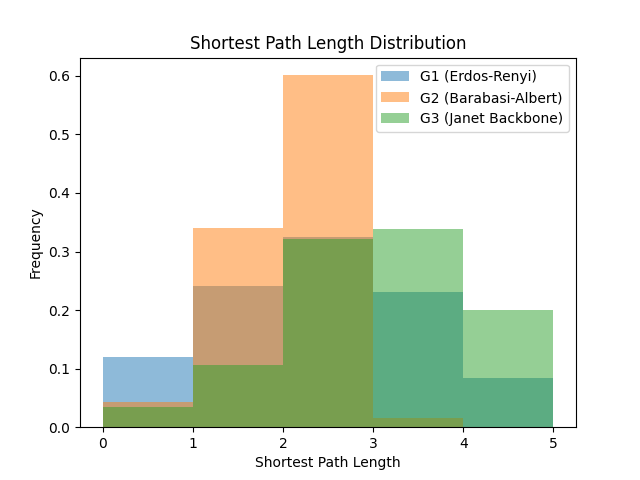
\includegraphics[width=.3\textwidth]{images/topo_comparison/janet2.png}\hfill
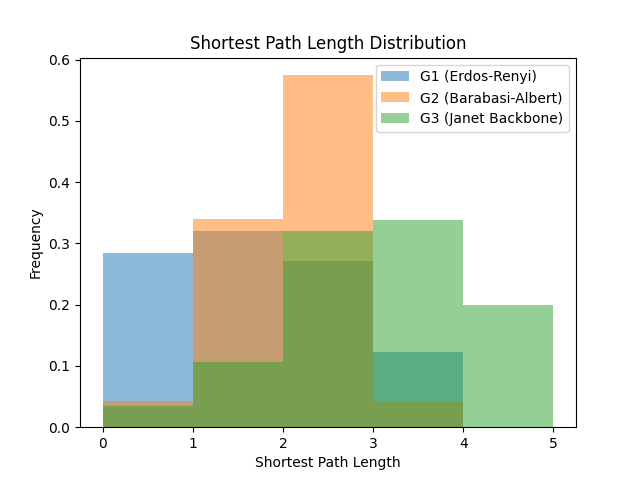
\includegraphics[width=.3\textwidth]{images/topo_comparison/janet3.png}
\caption{Shortest Path comparison between ER, BA and real-world Janet Backbone topology}
\label{fig:shortest_path_comp}
\end{figure}


\subsection{Virtual Lab implementation}

\subsubsection{NetworkX}
%Describe framework
NetworkX is a python library which is designed to be used for the "creation, manipulation, and study of the structure dynamics, and functions of complex networks." \cite{networkX} Due to it's extensive functionality, utilising this library for the evaluation and processing of graph topologies increases the speed and ease with which it can be carried out. Furthermore, as a consequence of it's robust implementation and over 90\% test coverage of it's code-base, results yielded utilising this library are highly trustworthy. 

%Modules used from framework
For the generation of random graph topologies, namely Erdos-Renyi and Barabasi-Albert, the corresponding modules are used; \newline
\verb|erdos_renyi_graph(n, p, seed=None, directed=False)| 
\verb|barabasi_albert_graph(n, m, seed=None, initial_graph=None)| 

For the comparison between the various topologies the following modules were used; \newline 
\verb|all_pairs_shortest_path_length(G, cutoff=None)|
%Code excerpt



\subsubsection{Oracle VM VirtualBox}
% Virtual environment allows greater portability
Oracle VM VirtualBox is an open source cross-platform virtualization software using a Type 2 hypervisor. \cite{VirtualWare} It's ease of installation and use on all of the major Operating Systems including Microsoft Windows, macOS, Linux, Solaris and OpenSolaris \cite{oracleVM} allows for high portability and cohesion. 

Due to the traceroute tools being developed for a Linux based operating system, VirtualBox is being used to host a Linux distribution on a windows machine without the need for a dual-boot or separate computer.

\subsubsection{Docker}
% Outline docker, and containers
Docker allows application images to be deployed in isolated containers \cite{docker_isolate}. This avoids the potential computational overhead of running an operating system using a virtual machine, and also allows for ease of deployment. It can be built into new and existing pipelines for automatic CI/CD, which is particularly advantageous in industry contexts. 

\subsubsection{ContainerLab}

% Outline containerlab, various topologies employed
ContainerLab builds upon the containerisation technology which docker provides. It centers on Network Operating Systems which are commonly used commercially and for network testing and diagnostics. This provides a more realistic testing environment which reflects real-world networks. Furthermore, it also allows a wide range of possible configurations between multiple different nodes running different Network Operating Systems.

\begin{figure}
    \centering
    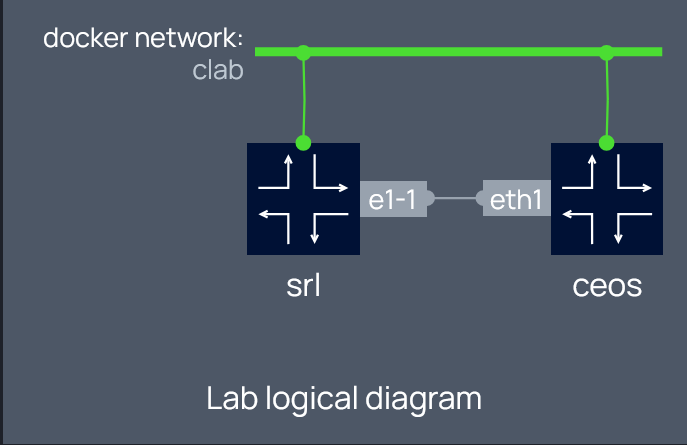
\includegraphics[width=0.5\linewidth]{images/lab_logical_diagram.png}
    \caption{Example Lab logical diagram \cite{containerlab}}
    \label{fig:lab_diagram_example}
\end{figure}

Configuration and management is controlled through a command-line interface (CLI), with the virtual topologies being defined straightforwardly in human readable YAML format. The topology is defined as "a set of nodes and links between them" \cite{containerlab}. Each of the nodes contains a kind to specify/control node behaviour, additionally each node also has an image link to the Network Operating System image to be loaded. The structure of the network is determined through a set of endpoints, expressing how each node is connected.

\begin{figure}
    \centering
    \begin{lstlisting}
name: srlceos01

topology:
  nodes:
    srl:
      kind: nokia_srlinux
      image: ghcr.io/nokia/srlinux
    ceos:
      kind: arista_ceos
      image: ceos:4.32.0F

  links:
    - endpoints: ["srl:e1-1", "ceos:eth1"]
\end{lstlisting}
    \caption{Example ContainerLab network topology defined in YAML file}
    \label{fig:topology_yml}
\end{figure}

Upon deployment of the lab, the lifecycle can be managed through deploy, destroy, save, inspect and graph operations. Further increasing it's utilitiy and usability as a virtual network lab.

\begin{figure}
    \centering
    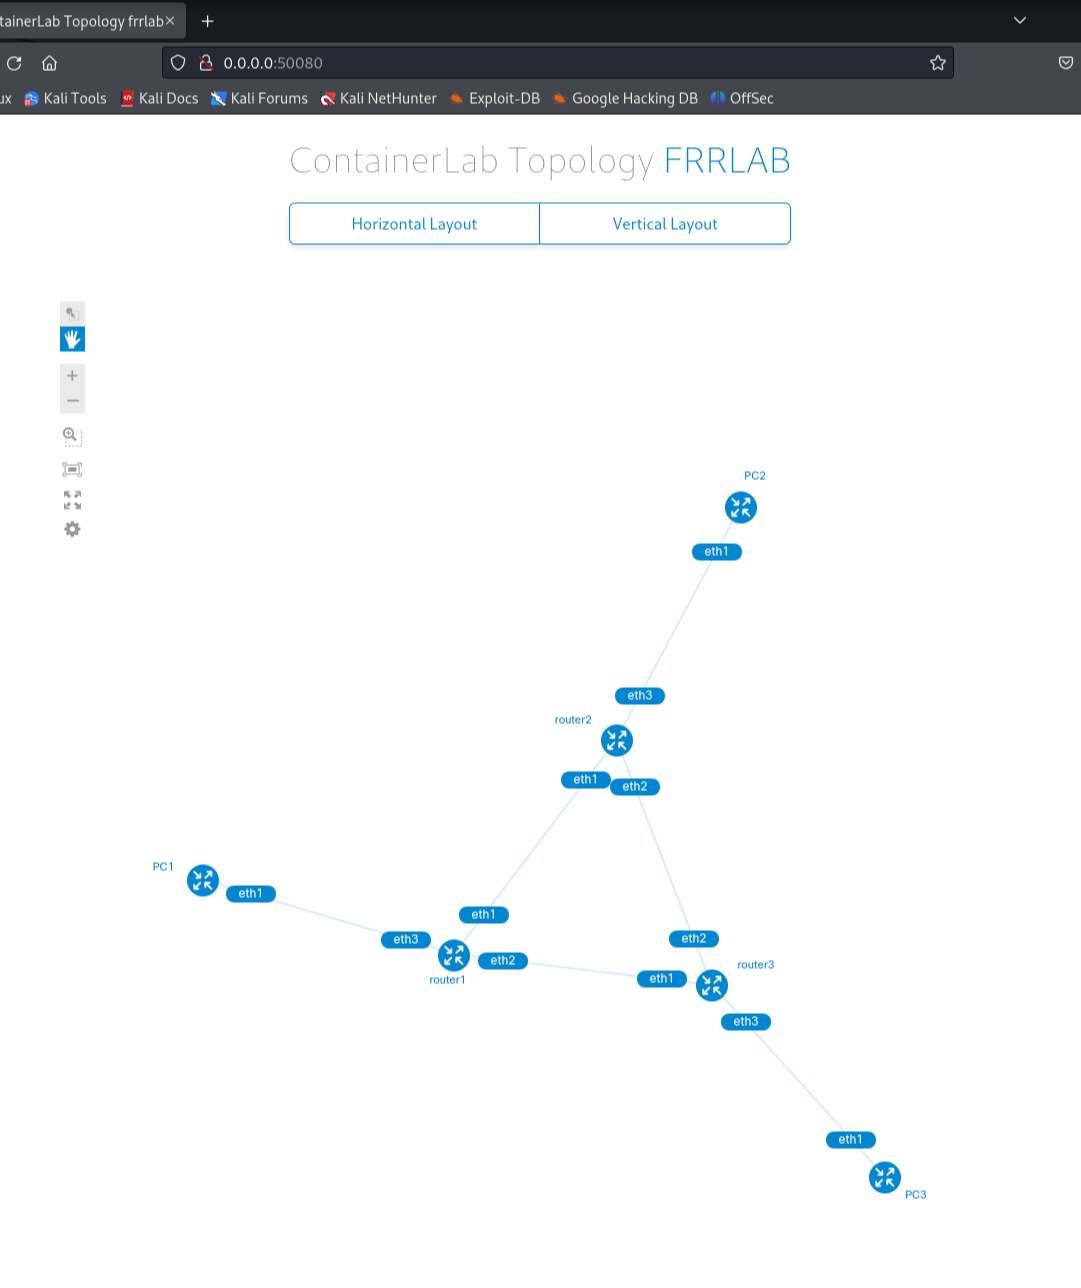
\includegraphics[width=0.5\linewidth]{images/ring_containerlab.png}
    \caption{Containerlab network topology visualisation feature, showing a simple ring network structure.}
    \label{fig:ring_container}
\end{figure}

\subsubsection{Alpine Linux}
% Lightweight distro
For the implemented virtual network lab, Alpine Linux has been used due to it's small size and resource efficiency. When installed on a container, it  requires a minimal 8 MB of space \cite{alpine}. However, this reduction of space overhead has a trade-off; an instance of this is that Apline uses a non-regular package manager called apk; this has proved to be problematic during creation of the network lab, due to lack of support to install the required network scanning libraries on containers to facilitate testing. 

\subsubsection{Virtual network pipeline}
As previously mentioned, to facilitate simulation of the randomly generated network topologies, the generated structures could be parsed into the YAML format required for containerlab to deploy virtual networks. Implementation of a seamless "pipeline" is of great benefit as it allows modular steps in the creation of the network lab to be connected linearly, allowing straightforward configuration and control of each step in the process. Furthermore, it also has the additional benefit of being more extensible and resilient to bugs and anomalies as these can be isolated at specific stages in the pipeline. An additional benefit is ease of use, should the framework be adopted in the future for further research. Below, a framework is proposed with the aim of accomplishing this; from the initial generation of network topologies to the simulation and evaluation of them using configurable contemporary methods. 

topology generation $\Rightarrow$ parsing to YML $\Rightarrow$ deployment of containerlab environment $\Rightarrow$ selection of network scanning method $\Rightarrow$ running scan on deployed topology $\Rightarrow$ evaluating scan using configurable metric 

To facilitate simulation of real-world topologies from the Internet Topology Zoo dataset, a similar pipeline is proposed. In which the GML graph files are parsed to YML format, which are then deployed using containerlab, continuing onto be scanned using a chosen scanning method and evaluated using a configurable metric.  

Topology selection from Dataset $\Rightarrow$ parsing to YML $\Rightarrow$ deployment of containerlab environment $\Rightarrow$ Selection of scanning method $\Rightarrow$ running scan on deployed topology $\Rightarrow$ evaluating scan using configurable metric 

% Create diagrams for each step in pipeline, with accomanying code to go with each step. 

\subsubsection{Proposed topologies}
6 topologies are proposed to be used to evaluate each of the network scanning methods, with 3 being randomly generated and 3 being from real-world topologies. Each topology has been selected from larger topology sets as outline in previous sections, with the intention of providing a diverse range of structures with which to test the scanning tools. This approach does have limitations however, including selection bias, and a relatively small number of test-cases. 

%compare the generated networks and real-world networks r value, as a measure of correlation and therefore relavance in testing the network scanning tools

\subsection{Network scanning methods}
Below, the performance on both real-world and randomly generated topologies will be outlined for each network scanning tool. 

\subsubsection{Original traceroute (Jacobson's)}



\subsubsection{Paris traceroute}

\subsubsection{Dublin traceroute}

\subsection{Proposed Algorithms}
Below, the proposed algorithms Zeph and MDA are outlined and described. They are suggested as possible extensions to the Dublin-traceroute tool to improve it's performance.  

\subsubsection{Zeph algorithm}

\begin{algorithm}
\caption{Zeph Algorithm}\label{alg:zeph}
\begin{algorithmic}[1]
\State \textbf{Input:} Graph $G(V, E)$, source node $s$, destination node $t$
\State \textbf{Output:} Shortest path from $s$ to $t$
\State Initialize priority queue $Q$ and set $Q = \{(s, 0)\}$
\State Initialize distance vector $D$ with $D[s] = 0$ and $D[v] = \infty$ for all $v \neq s$
\While{$Q$ is not empty}
    \State Extract $(u, d_u)$ from $Q$ with the smallest $d_u$
    \If{$u == t$}
        \State \textbf{return} $D[t]$
    \EndIf
    \For{each neighbor $v$ of $u$}
        \State Calculate tentative distance $d_{tentative} = d_u + w(u, v)$
        \If{$d_{tentative} < D[v]$}
            \State Update $D[v] = d_{tentative}$
            \State Insert $(v, D[v])$ into $Q$
        \EndIf
    \EndFor
\EndWhile
\State \textbf{return} $D[t]$ \Comment{If $t$ is unreachable, $D[t]$ will be $\infty$}
\end{algorithmic}
\end{algorithm}

\subsubsection{ MDA/MDA-lite}

DOUBLE CHECK THIS
\begin{algorithm}
\caption{MDA: Modularity Density Algorithm}\label{alg:mda}
\begin{algorithmic}[1]
\State \textbf{Input:} Graph $G(V, E)$, modularity parameter $\gamma$
\State \textbf{Output:} Optimal community structure $C$
\State Initialize community structure $C_0$ with each node in its own community
\State Initialize modularity density $\Delta Q = 0$

\Repeat
    \State Calculate the modularity density $\Delta Q$ for current community structure $C$
    \For{each node $i \in V$}
        \State Compute the potential gain in modularity density by moving node $i$ to a neighboring community
        \If{gain in $\Delta Q > 0$}
            \State Move node $i$ to the community that provides the maximum increase in $\Delta Q$
        \EndIf
    \EndFor
\Until{no further improvement in modularity density is possible}

\State \textbf{Output} the community structure $C$ that maximizes modularity density $\Delta Q$
\end{algorithmic}
\end{algorithm}

\newpage

\subsection{Data Processing}

\subsubsection{Pandas}

\subsubsection{Matplotlib}
